\documentclass[12pt,titlepage]{report}
\usepackage[authoryear,semicolon]{natbib}
\usepackage{mathptmx} 
\usepackage{pdfpages}
%\usepackage{chicago}
\usepackage[onehalfspacing]{setspace}
%\doublespacing
%\linespread{1.6}
\setstretch{1.5}
%\usepackage{figure}
\onehalfspacing
\usepackage[left=40mm,right=25mm,top=30mm,bottom=20mm,headsep=10mm]{geometry}
\geometry{a4paper}
\usepackage[titletoc]{appendix}
\usepackage{fnpara}
\usepackage{graphicx}
\usepackage{epstopdf}
%\usepackage{mathtools}
\usepackage{amsmath,amsfonts,amsthm,amssymb}
\usepackage{fancybox}

%\usepackage[active]{srcltx}
\usepackage{afterpage}
\usepackage[mathscr]{eucal}
\DeclareGraphicsRule{.tif}{png}{.png}{`convert #1 `dirname
#1`/`basename #1 .tif`.png}
%\usepackage{fancyhdr}
%\pagestyle{fancy}
%\fancyhf{}
%\rhead{ \leftmark}
%\rhead[\thepage]{\chaptermark}
%\lhead{Oyebamiji, O.K.}
%\cfoot{ \thepage}


\usepackage{setspace}
\usepackage[small]{caption}
\usepackage{color}
\usepackage{apalike}
%\usepackage{subcaption}
\usepackage{placeins}
\usepackage{epstopdf}
\usepackage{booktabs}
\usepackage{tikz}
\usepackage{subcaption}
%\usepackage{color,framed} %Utilisation des couleurs et de l'environnement shaded
%\definecolor{shadecolor2}{rgb}{.92,.92,.92} % choix de la teinte de ``shaded''
%\definecolor{shadecolor}{rgb}{.6,.95,.6} % choix de la teinte de ``shaded''
\usepackage[pagebackref=true,colorlinks=true, linkcolor=blue,anchorcolor=blue,citecolor=blue,filecolor=blue,menucolor=blue,
urlcolor=black,plainpages=false,pdfpagemode=UseThumbs,pdftitle={Titre},pdfauthor={oluwole},
pdfsubject={Thesis},pdfstartview=FitH]{hyperref} % Extensions PDF
%\def\pdfBorderAttrs{/Border [0 0 0] } % Options PDF (No border around Links)
%\usepackage[plainpages=false,backref=page,hypertexnames=true,linktocpage=true,colorlinks=true,citecolor=blue,linkcolor=blue]{hyperref}


%=========Standard sets===========:
\newcommand{\stsets}[1]{\mathbb{#1}}
\newcommand{\R}{\stsets{R}}
\newcommand{\N}{\stsets{N}}
\newcommand{\C}{\stsets{C}}

%===============Theorems etc.========================
%Paul
\newcommand{\bt}{{\bf t}}
\newcommand{\bB}{{\bf B}}
\newcommand{\bSigma}{{\bf \Sigma}}
\newcommand{\tbSigma}{{\tilde {\bf \Sigma}}}
\newcommand{\tbu}{{\tilde {\bf u}}}
\newcommand{\tbU}{{\tilde {\bf U}}}
\newcommand{\bh}{{\bf h}}
\newcommand{\bH}{{\bf H}}
\newcommand{\bD}{{\bf D}}
\newcommand{\bU}{{\bf U}}
\newcommand{\bu}{{\bf u}}
\newcommand{\bZ}{{\bf Z}}
\newcommand{\bz}{{\bf z}}
\newcommand{\bC}{{\bf C}}
\newcommand{\bc}{{\bf c}}
%%
\newcommand{\bx}{{\bf x}}
\newcommand{\bX}{{\bf X}}
\newcommand{\by}{{\bf y}}
\newcommand{\bY}{{\bf Y}}
\newcommand{\bE}{{\bf E}}
\newcommand{\bW}{{\bf W}}
\newcommand{\tbx}{{\tilde {\bf x}}}
\newcommand{\tbX}{{\tilde {\bf X}}}
\newcommand{\tby}{{\tilde {\bf y}}}
\newcommand{\tbY}{{\tilde {\bf Y}}}
\newcommand{\hbX}{{\hat {\bf X}}}
\newcommand{\hbY}{{\hat {\bf Y}}}
\newcommand{\hby}{{\hat {\bf y}}}
\newcommand{\ty}{{\tilde {y}}}
\newcommand{\hy}{{\hat {y}}}
\newcommand{\bs}{{\bf s}}


\newcommand{\bLambda}{\mathbf{\Lambda}}
\newcommand{\bGamma}{\mathbf{\Gamma}}
\newcommand{\hbGamma}{\hat {\mathbf{\Gamma}}}

\newcommand{\bgamma}{{\boldsymbol{\gamma}}}
\newcommand{\bepsilon}{{\boldsymbol{\varepsilon}}}
\newcommand{\tbepsilon}{{\tilde{\boldsymbol{\varepsilon}}}}
\newcommand{\hbepsilon}{{\hat{\boldsymbol{\varepsilon}}}}
\newcommand{\bbeta}{{\boldsymbol{\beta}}}
\newcommand{\hbbeta}{{\hat{\boldsymbol{\beta}}}}
\newcommand{\btau}{{{\boldsymbol{\tau}}}}
\newcommand{\balpha}{{\boldsymbol{\alpha}}}
\newcommand{\bhalpha}{{\hat{\boldsymbol{\alpha}}}}


\theoremstyle{definition}
\newtheorem{definition}{Definition}
\theoremstyle{remark}
\newtheorem{remark}[definition]{Remark}
\newtheorem{example}[definition]{Example}

%\newtheoremstyle{mytheorem}{0.5cm}{0.2cm}{\slshape}{ }{\bfseries}{.}{}{}
%\theoremstyle{my theorem}
\newtheorem{Th}[definition]{Theorem}
%\newtheorem{Prop}[definition]{Proposition}
\newtheorem{lemma}[definition]{Lemma}
\newtheorem{Cor}[definition]{Corollary}
%\restylefloat{figure}

%==========Probabilistic===========:
%\renewcommand{\cite}{\shortciteN}
\renewcommand{\P}{\mathbf{P}}
\renewcommand{\Re}{\mathrm{Re\,}}
\renewcommand{\Im}{\mathrm{Im\,}}
%\newcommand{\Prob}[1]{\mathbf{P}\{#1\}}
\DeclareMathOperator{\E}{{\bf E}}
\DeclareMathOperator{\var}{{\bfvar}}
\DeclareMathOperator{\supp}{supp}
\DeclareMathOperator{\dist}{dist}
\DeclareMathOperator{\one}{{1\hspace*{-0.55ex}I}}
%\DeclareMathOperator{\one}{{\mathbf{1}}}
\newcommand{\Ind}[1]{\one_{#1}}
\newcommand{\cond}{\hspace*{1ex} \rule[-1ex]{0.15ex}{3ex}\hspace*{1ex}}

%==========Divers===========:
\DeclareMathOperator*{\ssum}{{\textstyle \sum}}
%small\sum for\sum\delta_x
\newcommand{\comp}{\mathbf{c}}
\newcommand{\mydot}{{\raisebox{.3ex}{$\scriptscriptstyle{\,\bullet\,}$}}}
%\newcommand{\myline}{\newline\underline{\hskip\textwidth}}
\newcommand{\mytimes}{\!\times\!}
\newcommand{\mytilde}{{\!\raisebox{-0.9ex}{$\tilde{\ }$}}}
\renewcommand{\epsilon}{\varepsilon}
\renewcommand{\vec}[1]{\mathbf{#1}}
%\renewcommand{\phi}{\varphi}
\newcommand{\ti}{\to\infty}
\newcommand{\ssp}{\hspace{2pt}}
\newcommand{\seg}{see, \hbox{e.\ssp g.,}\ }
\newcommand{\ie}{\hbox{i.\ssp e.}\ }
\newcommand{\eg}{\hbox{e.\ssp g.,}\ }
\newcommand{\cf}{\hbox{c.\ssp f.}\ }
\newcommand{\etc}{\hbox{etc.}\ }
\newcommand{\iid}{\hbox{i.\ssp i.\ssp d.}\ }
\newcommand{\as}{\hbox{a.\ssp s.s}\ }
\newcommand{\viz}{\hbox{viz.}\ }
\renewcommand{\bibname}{References}
\renewcommand{\abstractname}{Abstract}


%\pagenumbering{roman}

\begin{document}
\chapter{Emulation of LAMMPS outputs}
We describe the procedure for building a simple emulator of LAMMPS output.
%\section*{LAMMPS emulator}
\section{Experimental design}
This section describes the procedure for generating the parameter combinations and variables at which the LAMMPS model is run. We run the LAMMPS code for a small sample of inputs using a Latin Hypercube Design (LHD). The design produces data for training the LAMMPS emulator to approximate the major LAMMPS outputs. LHD provides a good coverage of the input space with a relatively small number of design points. We use maximin LHS technique that optimises samples by maximizing the minimum distance between design points \citet{pd5}. Suppose we want to sample a function of $p$ variables, the range of each variable is divided into $n$ reasonable intervals, $n$ sample points are then drawn such that a Latin Hypercube is created.

We generate an $n \times p$ variables Latin Hypercube sample matrix with values uniformly distributed on interval [0,1]. We then transformed the generated sample to the quantile of a uniform distribution using the range of the parameters given in Table \ref{mytab1}.  LAMMPS model is computationally demanding, we limit our initial analysis to just $n=100$ training points for each dimension of the $p=22$ input spaces that are to be varied. %The inversion of the correlation matrix under GP regression becomes more difficult as we increase the number of training points. 

%(in this report, we consider only mean floc diameter)

\begin{figure}[!ht]
%\centering
\begin{subfigure}[b]{.5\textwidth}

\includegraphics[height=.4\textheight]{image1000001}
\caption{time t=0)}
\label{}
\end{subfigure}%\vspace*{-.1em}
%\centering
\begin{subfigure}[b]{.5\textwidth}

\includegraphics[height=.4\textheight]{image1000050}
\caption{time t=100000}
\label{}
\end{subfigure}\vspace*{-.1em}
% \centering
\begin{subfigure}[b]{.5\textwidth}
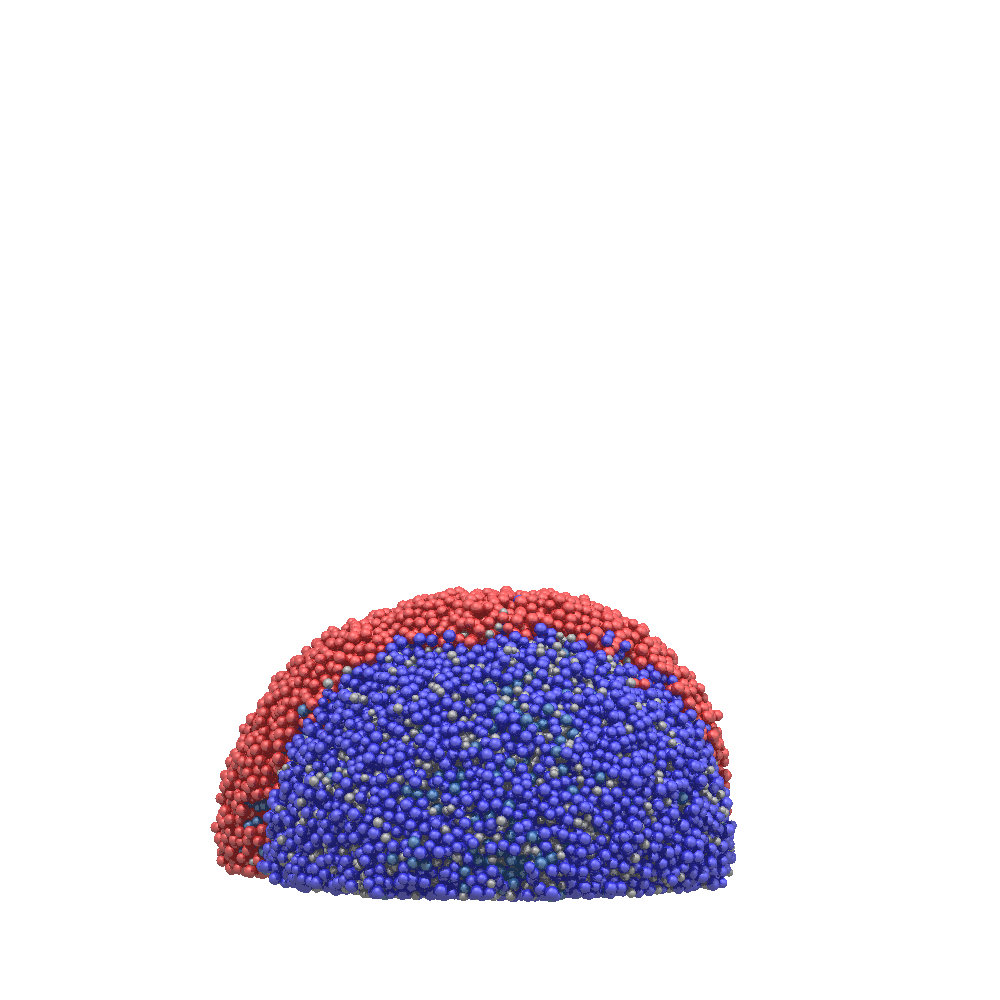
\includegraphics[height=.4\textheight]{image1000150}
\caption{time t=300000}
\label{}
\end{subfigure}\vspace*{-.1em}
%\centering
\begin{subfigure}[b]{.5\textwidth}
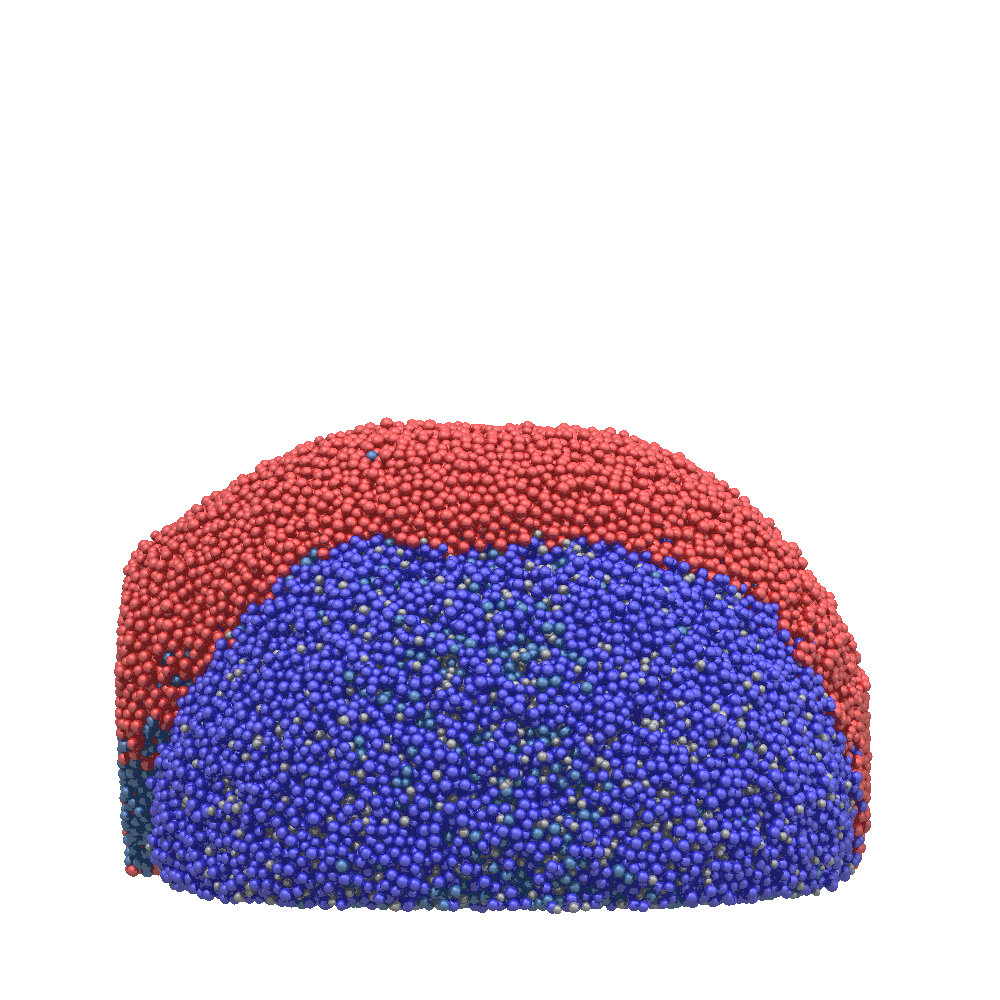
\includegraphics[height=.4\textheight]{image1000175}
\caption{time t=350,000}
\end{subfigure}\vspace*{-.1em}
\caption{Sample of LAMMPS simulation data for particle growth for 4 different time points (seconds).}\label{myfig1}
\end{figure}


\subsection{Simulation data}
We describe two different simulation procedures. Firstly, let the design matrix which contain the input to the LAMMPS model be denoted by $D=(\theta^i_p, t_p, p=1,\ldots,22; i=1,\ldots,100)$, where the subscript $p$ represents the 22 input parameters and superscript $i$ denote 100 different realisations (design points), $t_p$ is the time in seconds at which the output data is recorded. The design matrix $D_{100 \times 23}$ denotes the input values at which the LAMMPS model will be run for every combinations of $x_p$ where $x_p$ represents $p^{th}$ row of $D$. The current LAMMPS code is set up to produce the following outputs namely particle diameter, position (3-dimensional), velocity (3-dimensional) and force (3-dimensional). The LAMMPS code could be run for as long as there are sufficient computing resources to store the outputs. For the present analysis, the code is run for 352800 seconds to generate sufficient data for the emulation that is equivalent to $\approx$ 4 days of real time and generated output results are saved at a time-step of 2000 seconds which gives about 176 different time slices. 

Therefore, a single run of the code for each of design point $x_p$ will produce ten different outputs and 176-time steps. There are 5 different types (or species) of the particle in the simulation namely AOB, NOB, HET, EPS and inert. We note that the shape and number of particles as well as the composition of the floc at each time step vary in the simulation. 

We perform the second simulation using the same input configuration as described above but repeated the runs for five times to incorporate stochastic variations in our outputs. The large design, of course, increases the amount of CPU time for the entire simulations even with running the bash script in parallel on a Linux machine. 


\section{Method 1: Combination of linear models and Gaussian process regression}
\subsection{Procedure}
We describe the analysis of the first dataset here.
The work focuses on predictions of mean floc diameter from LAMMPS simulation outputs together with their associated uncertainty levels. We propose a two-stage approach similar to \citet{pd11} where we shall combine a linear model in the first stage and a Gaussian process regression for residual interpolation in the second stage.

The step by step procedure for emulating one of the outputs of LAMMPS model, "particle floc diameter" is given here. We start by computing the average diameter of all the particles at each time step to obtain a vector $\by(x)=\bar z_1,\ldots,\bar z_{176}$ of the mean floc diameter to be emulated such that
\begin{equation}
\bar z_t=\frac{\sum^N_{k=1} z_{kt}}{N}
\end{equation}
where $k=1,\ldots, N$, $N$ represents the total number of all 5 particles at each time slice. We also note that $N$ varies across time point and in particular increases with time as seen in Figure \ref{myfig1} and $z_{kt}$ is a simulation floc diameter for particle $k$ at time $t$.

\subsection{Stage 1: Linear models}
For the training data, we sub-sample 75 out of 176-time slices for each design point $x_p$ which gives a total of 7500 observations.
The training data are ($7500 \times 1$) vector of mean floc diameter $\by$ of LAMMPS output and ($7500 \times 23$) matrix $\bX$, which holds the values taken by the explanatory variables. (NOTE: sequence of time $t$ at which output is sought is used as an additional input to the emulator). We fit a linear model to data $[\by,\bX]$ and then obtain the predictions $\hby$.
We also use the fitted model to predict the left out observations $\tby^{new}$ for cross-validation purpose and to obtain standard error of predictions $\bs^{new}$, which is a measure of prediction uncertainty in the linear model. 

%Finally, we apply a GP to model the residual field obtaining from the linear model.
In order to construct emulator for the prediction of mean particle diameter, we apply a standard regression to the data in the first stage using equation (\ref{geneq}) and use a Gaussian process regression for interpolating unexplained residual from linear model
\begin{equation}\label{geneq}
\by=f(\textbf{\bx})+\boldsymbol\varepsilon= \beta'_0+\beta'_{1}x_{1}+\ldots +\beta'_{p}x_{p}+\boldsymbol\varepsilon
\end{equation}
where $\by$ is the LAMMPS simulated mean floc diameter, $p=23$ is the number of parameters for estimation and $\bx_1,\ldots,\bx_p$ are independent variables and $\beta'_1,\ldots,\beta'_{23}$ are regression coefficients. We assume $\boldsymbol \varepsilon \sim N(0, \sigma^2)$. 

\subsection{Summary of steps taken for stage 1 modelling}
\begin{itemize}
\item[{(i)}] Design of experiment to identify important outputs (which outputs are to be emulated). 
\item[{(ii)}] Determine the relevant input factors to be varied (use all the 22 factors for now). 
\item[{(iii)}] Assign uniform probability density to each input variable (we have little knowledge about these parameters). 
\item[{(iv)}] Generate LHS of 100 design points on each of the 22 input parameters and transform into the quantile of uniform distribution using parameter ranges in Table \ref{mytab1}. 
\item[{(v)}] Evaluate LAMMPS model for various input combinations to obtain the training data.
\item[{(vi)}] Compute the LAMMPS mean floc diameter for each time-step from output data
\item[{(vii)}] Randomly sample 75 time points out of 176 for each design point
\item[{(viii)}] Fit a linear model with equation (\ref{geneq}) using all 23 parameters (time is included as an additional variable to the linear model)
\item[{(ix)}] Obtain both predictions and standard error of predictions for all data points
\end{itemize}

\subsection{Stage 2: GP modelling of residual data}\label{GP}
The (${7500\times 1}$) vector of residual $\boldsymbol \varepsilon=\by-\hby$ obtained from stage 1 formed our new training data in this section. This residual can be modelled as $\boldsymbol \varepsilon= \eta(X')$. We do not apply GP to all the 23 input variables in stage 1. Rather, we use standardized regression coefficients of equation (\ref{geneq}) as a measure of sensitivity to select important explanatory variables for the GP regression such that $X'<< X$ (ie $p$ is now $<23$).
Since Gaussian process is described completely by its mean and covariance functions, the mean function is given as
\begin{equation}\label{eqgp3}
E[\eta(X')|\boldsymbol\beta]=h^{\rm T}(\bX')\boldsymbol\beta,
\end{equation}
where $h(\bX')$ is a vector of regression functions. For our analysis, we use a simple linear function $h(\bX') = (1,\bx^T$) and $\boldsymbol\beta$ is an unknown hyperparameter to be estimated and covariance function $$ K={Cov[\eta(\bx),\eta(\bx')|\sigma^{2},\boldsymbol \alpha]=\sigma^{2} \bC(\bx,\bx^{\rm T})},$$ where $\sigma^{2}$ is a noise variance and $\bC(\bx,\bx^{\rm T})$ is a correlation function with an hyperparameter $\boldsymbol \alpha$. We use a Gaussian correlation function of the form
\begin{equation}\label{gaus}
\bC=\Big \{\exp(-(x-x')^T \boldsymbol \alpha (x-x')) \Big\},%\exp^{\Big[\sum \limits_{j=1}^{4}{-\boldsymbol \alpha_j(\bx_{j}-\bx^{\rm T}_{j})^2}\Big]}.
\end{equation}
where $\boldsymbol \alpha$ is the correlation hyperparameters to be estimated from the data. It is difficult to apply a GP directly to the entire residual data because of the inversion of covariance matrix which scales cubically with the number of
observations O($N^3$), we proceed by sub-sampling just 200 random observations from the data and denote the training data as $[\by, \bX']$, where $\by=[ \varepsilon_1= \eta(x_1),\ldots, \varepsilon_{200}= \eta(x_{200})]$. We select just 4 important explanatory variables for the GP modelling and our correlation parameter is denoted as $\boldsymbol \alpha=(\alpha_1,\ldots,\alpha_4)$.

For computing the posterior distribution, we assign a non-informative prior to the $\boldsymbol \beta$, $\sigma^2$ and $\alpha$ parameters such that $p(\bbeta, \sigma^2) \sim \sigma^{-2}$ and $p(\alpha) \sim 1$.
To obtain the posterior estimates using Bayes theorem, we update these prior distributions on some data $\by$. We estimate their values by conditioning on each parameter and maximize the resulting marginal likelihood function \citep{pd7,pd10}. Therefore, the resulting posterior distribution is denoted as $\eta(.)|\by \sim N\Big \{\mu^{\star}, K^{\star} \Big\}$, where

\begin{equation}\label{olu1}%\tag{A.8}\label{olu1}
\mu^{\star}(\mathbf{x})=h(\mathbf{x})^T\boldsymbol{\hat\beta}+t(\mathbf{x})^T\bC^{-1}[\by-\bH\boldsymbol{\hat\beta}]
\end{equation}
\begin{multline}\label{olu2}%\tag{A.9}\label{olu2}
\begin{split}
K^{\star}=\hat \sigma^2 \Big \{c(\mathbf{x,x'}) -t(\mathbf{x})^T\bC^{-1} t(\mathbf{x}) + \\ \Big ( h(\mathbf{x})^T-t(\mathbf{x})^T\bC^{-1}t(\mathbf{x}) \Big )
(\bH^T\bC^{-1}\bH)^{-1}\Big ( h(\mathbf{x'})^T-t(\mathbf{x'})^T\bC^{-1}t(\mathbf{x'}) \Big )^T
\Big \}
\end{split}
\end{multline}
where $t(\bx)^T=[c(\bx,\bx_1),\ldots, c(\bx,\bx_n)]$ and $\bH^T=[h(\bx_1),\ldots, h(\bx_n)]$, see more details in the appendix. We analyse our results using $emulator$ package in $R$.

Finally, let the GP posterior mean and variance estimates of the residual at a new input point $x^{new}$ (cross-validation) be denoted as $\mu^{\star \star}$ and $K^{\star \star}$ respectively, and predictions and standard error of predictions from linear model as $\tby^{new}$ and $\bs^{new}$ respectively. The final predictions of mean particle diameter $\hby^{new}$ is given as
\begin{equation}\label{r1}
\hby^{new} = \tby^{new} +\mu^{\star \star}(\bx)
\end{equation}
and total uncertainty is
\begin{equation}\label{r1}
\hat \bs^{new} = \bs +\sqrt{|K^{\star \star}}|
\end{equation}

\subsection{Summary of stage 2}
\begin{itemize}
\item[{(i)}] Perform the GP emulation of the unexplained residual data 
\item[{(ii)}] Given the posterior density of $\alpha$ as defined in equation (\ref{like3}) of Appendix 1, compute the MLE of $\balpha$, such that equation (\ref{like3}) is maximized.
\item[{(iii)}] Set $\bC= \bC(\bhalpha)$
\item[{(iv)}] Compute estimate $\hbbeta=(\bH^T\bC^{-1}\bH)^{-1}\bH^T\bC^{-1}\by$
\item[{(v)}] Compute estimate $\widehat{\sigma^2}=\frac{1}{n-p}\Big[\mathbf{(y-H\hat{\boldsymbol \beta})}^T\bf C^{-1}(\bf y-H\hat{\boldsymbol \beta})\Big]$
\item[{(vi)}] Compute posterior mean estimate $\mu^{\star}(\mathbf{x})$ given in equation (\ref{olu1})
\item[{(vii)}] Compute posterior variance estimate $K^{\star}$ given in equation (\ref{olu2}) above
\end{itemize}

\begin{figure}[!ht]
\begin{subfigure}[b]{.5\textwidth}
%\centering
\includegraphics[height=10cm,width=1.1\textwidth]{res_plots/wole1}
\caption{LAMMPS and model predictions (emulator) for some randomly selected points}
\label{myfigg9a1}
\end{subfigure}\hspace*{1em}
\begin{subfigure}[b]{.5\textwidth}
%\centering
\includegraphics[height=10cm,width=1.1\textwidth]{res_plots/wole2}
\caption{LAMMPS and model predictions (emulator) for some randomly selected points}
\label{myfigg9a1}
\end{subfigure}
\begin{subfigure}[b]{.5\textwidth}
%\centering
\includegraphics[height=10cm,width=1.1\textwidth]{res_plots/wole3}
\caption{LAMMPS and model predictions at $79^{th}$ design point for all time steps}
\label{myfigg9a1}
\end{subfigure}\hspace*{1em}
\begin{subfigure}[b]{.5\textwidth}
%\centering
\includegraphics[height=10cm,width=1.1\textwidth]{res_plots/wole4}
\caption{LAMMPS and model predictions at $28^{th}$ design point for all time steps}
\label{myfigg9a2}
\end{subfigure}
\caption{Pair plot of model predictions (emulator) vs. LAMMPS values with their 95\% C.I for mean floc diameter (all species) from a two-stage technique}\label{myfig2}
\end{figure}


\chapter{Method 2: Kriging}
Having obtained the simulation data by running the LAMMPS model as described in the previous section, we describe an alternative emulation approach for fitting LAMMPS output data. This approach involves using a kriging model, where the two stage techniques describe in previous section are combined as a single step. Kriging is a geostatistical technique for interpolating the value of an unknown random observation from data $\by(\bx)$ observed at known locations. They are also commonly used for building cheaper surrogate model of expensive computer codes \cite{pd1,pd2, pd3,pd6}. Here, $\by(\bx)$ can be decomposed into a mixture of deterministic (non-random trend) and a residual random variation. The trend could be modelled as a constant in ordinary/simple kriging or as an $n^{th}$ order polynomial as in universal kriging. In this section, we shall discuss the universal kriging technique. The model formulation is given as
\begin{equation}\label{geneq2}
\by(\bx)= f(\bx) + \boldsymbol \varepsilon(\bx)
\end{equation}
where $\by(\bx)$ is as defined in equation (\ref{geneq}) above, $\boldsymbol \varepsilon(x)$ is a stationary Gaussian process with mean zero and known covariance function $K$. The deterministic function $f(\bx)$ is the mean approximation of the expensive computer simulator (eg LAMMPS) and $f$ is a polynomial function. Under this assumption, $f(x)$ can be modelled as
\begin{equation}
f(\bx) = \sum_{j=1}^{p} \beta_j h_j(x) =\bH(x) \bbeta
\end{equation}
$\bbeta=[\beta_1,\ldots,\beta_p]$ is a $(p\times 1)$ vector of unknown regression coefficients and $\bH(x) = [h_1(x), . . . , h_p(x)]^T$ is a $(n\times p)$ matrix of regression functions,
$\varepsilon(\bx)$ is a stochastic Gaussian process characterized by its covariance function
$K=Cov(\varepsilon(\bx),\varepsilon(\bx)) = \sigma^2\bC(\bx,\bx')$, where $\sigma^2$ denotes the variance of $\varepsilon(\bx)$ also called process variance and $\bC$ is a $(n\times n)$ positive definite matrix of correlation between $\varepsilon(\bx)$'s at the experimental design points.
Similarly, $\bt(x^{new}) = [Cor(x_1, x^{new}), \ldots,Cor(x_n, x^{new})]^T$ for the $(n\times 1)$ vector of correlations between the $\varepsilon(\bx)$'s at the design points and new input points $x^{new}$. We use both Gaussian equation (\ref{gaus}) and Matern correlation functions.
%\begin{equation}
%\bC(x,x')=\Pi^{p}_{j=1}\exp^{-\balpha(x-x')^2}, 
%\end{equation}
%with a parameter $\balpha$. 
The universal kriging predictor $\hby^(x^{new})$ of the value of $\by(x)$ at the new target point $x^{new}$ is the linear predictor
\begin{equation}
\hby(x^{new})=\sum_{j=1}^n \lambda_j \by (x_j)=\lambda(x)^T\by,
\end{equation}
for the sample points $x_1, \ldots , x_n$, where the coefficients or weights $\lambda=(\lambda_1, \ldots, \lambda_n)^T$ are estimated by minimizing the variance of prediction error for each realizations of the random function $\by(x)$. The best linear unbiased predictor (BLUP) is computed by minimizing the mean squared error
\begin{equation}\label{mse}
MSE[\hby(x^{new})]=E[\lambda^T\by-\by(x^{new})]^2,
\end{equation}
subject to the unbiasedness constraint $E[\lambda^T(x)\by] = E[\by(x^{new})]$. The mean squared error in equation (\ref{mse}) can be rewritten by substituting the value of $\by$ in equation (\ref{geneq2}), we thus have 
\begin{equation}
\sigma^2[1 + c\lambda^T(x)\bC\lambda(x) - 2\lambda^T(x)\bt(x^{new})],
\end{equation}
The unbiasedness constraint is now denoted as $H^T\lambda(x) = h(x)$. 
The optimal weights $\lambda^{*}_j$ in $\by(x^{new})$ is estimated by using Lagrange multipliers for constraining MSE minimization and solving system of equations in order to compute $p$ coefficients of $\lambda$.
If the inverse of matrix $\bC$ exists, then the best linear unbiased predictor for kriging model is given as
\begin{equation}
\hby_{uk}(x) = h^T(x)\hbbeta+ \bt^T(x)\bC^{-1}(\by -\bH\hbbeta)
\end{equation}
Similarly, by substituting in the optimal value of $\lambda^*(x)$ in the MSE equation, we have
\begin{multline}\label{olu2b}%\tag{A.9}\label{olu2}
\begin{split}
S^2_{uk}=\hat \sigma^2 \Big \{C(\bx,\bx') -\bt(\bx)^T\bC^{-1} \bt(\bx) + \\ \Big ( h(\bx)^T-\bt(\bx)^T\bC^{-1}\bt(\bx) \Big )
(\bH^T\bC^{-1}\bH)^{-1}\Big (h(\bx')^T-\bt(\bx')^T\bC^{-1}\bt(\bx') \Big )^T
\Big \}.
\end{split}
\end{multline}
See more details in \citep{pd4,pd5}
%where $\hbbeta$ is given below.%= (\bH^T\bC^{-1}\bH)^{-1}\bH^T\bC^{-1}\by$.

NOTE: Kriging technique is equivalent to the Bayesian method describes in section (\ref{GP}) if we assign improper uniform priors on the $\bbeta$. In other words, non-informative Bayesian analysis often leads to kriging predictor and variance and these estimators appear respectively as conditional mean and variance in equations (\ref{olu1} and \ref{olu2}).

We use a Maximum Likelihood Estimation (MLE) technique as an objective estimator of the kriging model parameters, $\theta=(\bbeta,\sigma^2,\boldmath \alpha)$. MLE assumes a Gaussian probability distribution. 
The likelihood of the model parameters is defined as the probability of the $n$ observations $\by= {y_1, …, y_n}$, given the model parameters such that 
\begin{equation}
L(\theta|\by)= \Pi_{j=1}^n p(\by_j|\theta).
\end{equation}
The expression for $L(\theta|\by)$ is given by equation (\ref{like}) below as
\begin{equation}\label{like}
L(\boldsymbol \beta, \sigma^2, \boldsymbol{\alpha};\by)\propto \frac{det(\bf C)^{-\frac{1}{2}}}{{(2\pi\sigma^2)}^\frac{n}{2}}\exp \Big \{\frac{(\by-H\boldsymbol \beta)^T \bf C^{-1}(\by-H\boldsymbol \beta)}{2\sigma^2}\Big\}
\end{equation}
where $\boldsymbol{\alpha}=[\alpha_1, \ldots, \alpha_n]$ is a vector of correlation lengths and $det(\bf C)$ is the determinant of correlation matrix $\bC$.
By taking the derivative of the log-likelihood of equation (\ref{like}) with
respect to $\bbeta$ and $\sigma^2$ and solving for zero, the estimates $\hbbeta$ and $\hat\sigma^2$ are given respectively as $\hbbeta=(\bH^T\bC^{-1}\bH)^{-1}\bH^T\bC^{-1}\by$ and $\hat{\sigma^2}=\frac{1}{n}\Big[\mathbf{(y-H\hat{\boldsymbol \beta})}^T\bf C^{-1}(\bf y-H\hat{\boldsymbol \beta})\Big]$.

In order to estimate $\balpha$, we maximize over $\balpha$ the concentrated likelihood given below after plugging the values of $\hbbeta$ and $\hat\sigma^2$
\begin{equation}
-2 log L(\hbbeta, \hat \sigma^2, \balpha; \by) = n log(2\pi) + n log\hat \sigma^2 + log(det(\bC)) + n
\end{equation}
The trend and covariance parameters $\theta$ are computed quickly and very efficiently by using a global optimiser which is based on the extension of efficient algorithm proposed in \cite{pd9} for likelihood maximization. See further details in \citep{pd8}.

\section{Kriging results}
Some results from kriging technique are given here. Recall from above that our training data are ($7500 \times 1$) vector of mean floc diameter $\by$ of LAMMPS output and ($7500 \times 23$) matrix $\bX$ of input variables. Here, we use the same 75 out of 176-time slices but we sub-sample just 50 design points to reduce further the dimension of the data which gives a total of 3750 observations. The new training data for the kriging model is $D=[\by_{3750 \times 1}, X_{3750 \times 23}]$. We fit the data using the $DiceKriging$ package in $R$. We consider only the linear terms for the trend model (no quadratic terms). We compare both Matern and Gaussian covariance functions with little difference in their predictions. The performance of the kriging emulator is tested by using the fitted model to predict the left out data. 

We also perform the sensitivity analysis of the mean particle floc diameter to identify relevant variables. We use a Sobol technique that involves decomposing total output variance as a summand of increasing dimensionality. We sampled 1000 observations from a uniform distribution for each of the 23 input variables in Table 1. We compute the sensitivity indices for three different methods. Bootstrapping was used to compute 95\% confidence intervals on the estimated indices.  The $sensitivity$ package was used for this analysis. The indices are shown in Figure \ref{sens} and we can see that only 4 parameters are relevant. Finally, we refitted the kriging model using just these four important parameters, some visual plots of results comparing the LAMMPS simulations with the emulator are showing in Figure \ref{myfig3}. We also compute the total percentage of variance explained by the final model that is $\sim 99\%$.



\begin{figure}[!ht]
\begin{subfigure}[b]{.5\textwidth}
%\centering
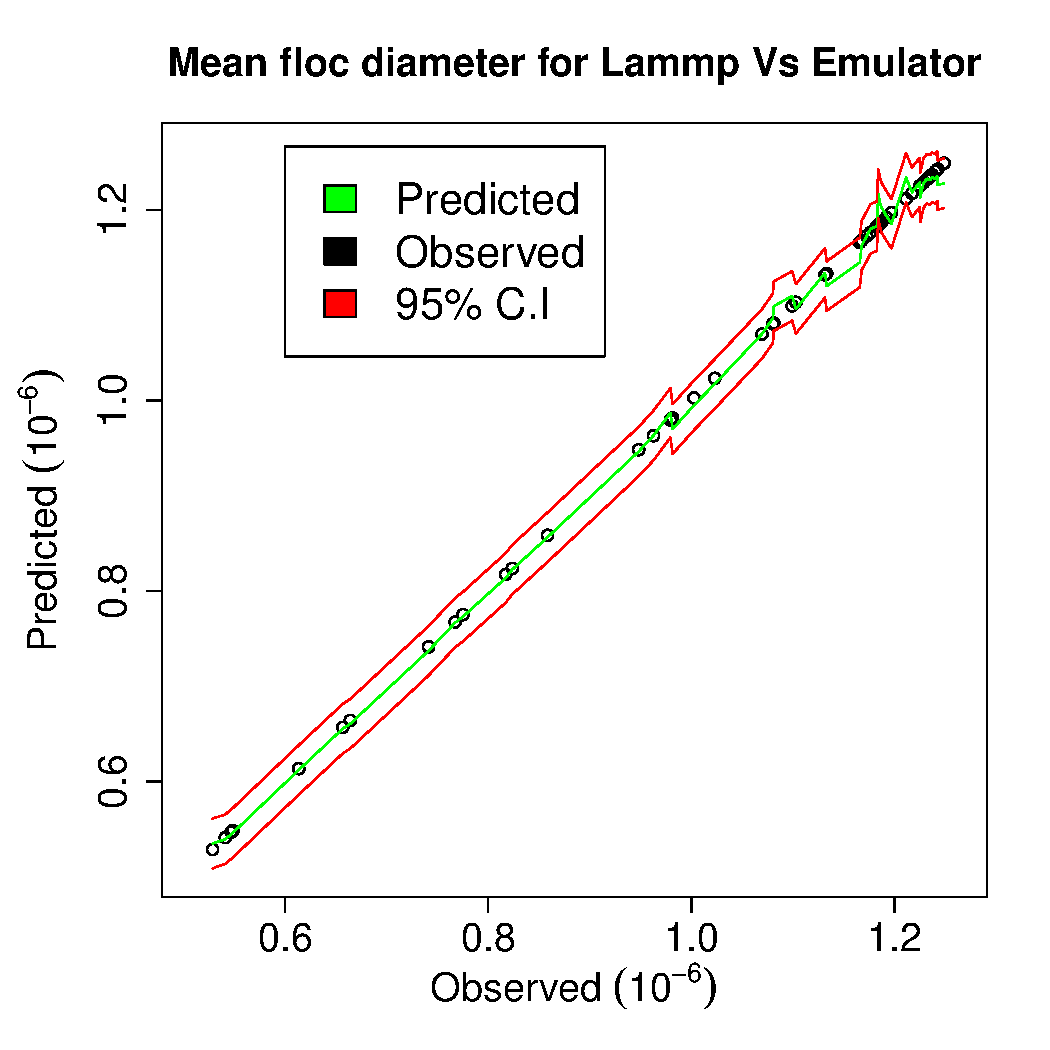
\includegraphics[height=9cm,width=1.1\textwidth]{ana/myplot1}
\caption{LAMMPS and kriging predictions (emulator) for some randomly selected points}
\label{myfigg9a1}
\end{subfigure}\hspace*{1em}
\begin{subfigure}[b]{.5\textwidth}
%\centering
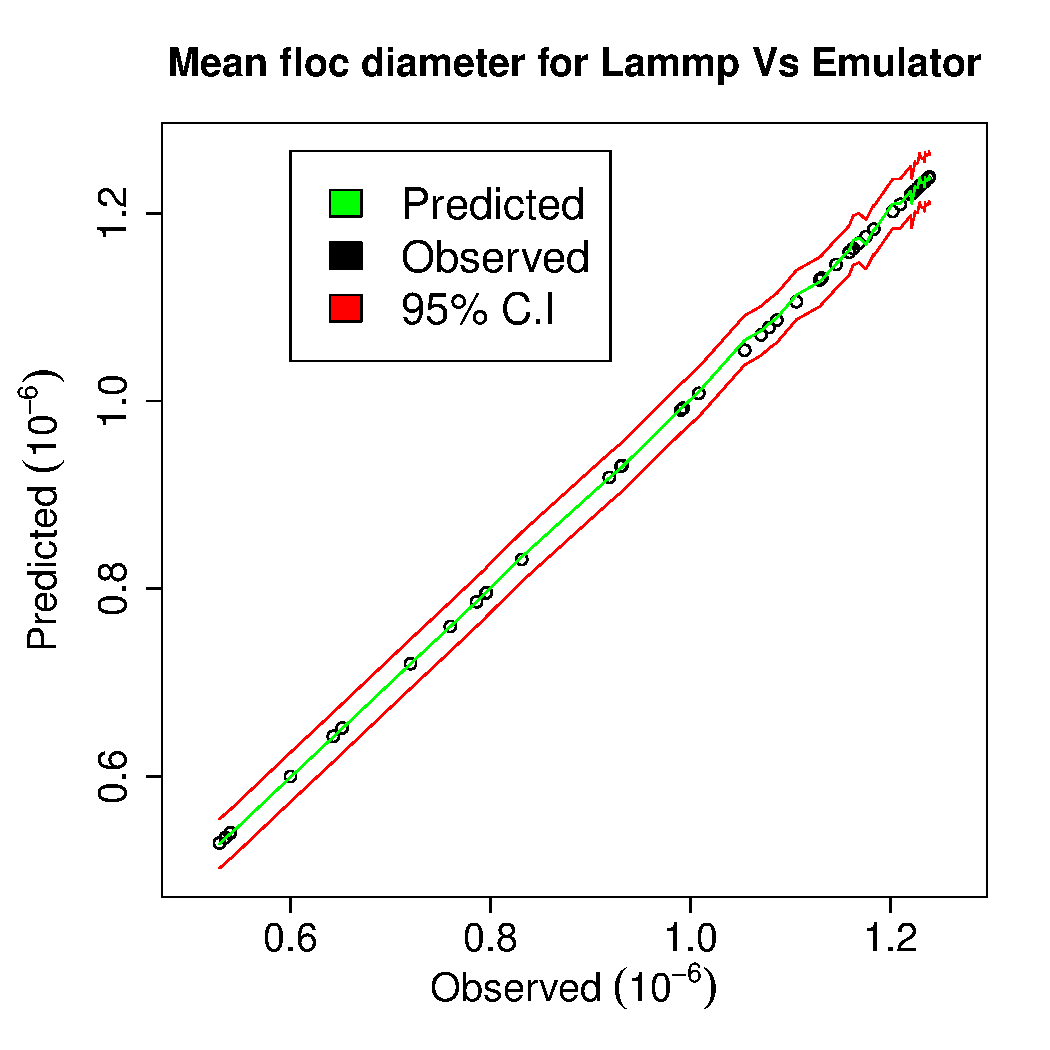
\includegraphics[height=9cm,width=1.1\textwidth]{ana/myplot2}
\caption{LAMMPS and kriging predictions (emulator) for some randomly selected points}
\label{myfigg9a1}
\end{subfigure}
\begin{subfigure}[b]{.5\textwidth}
%\centering
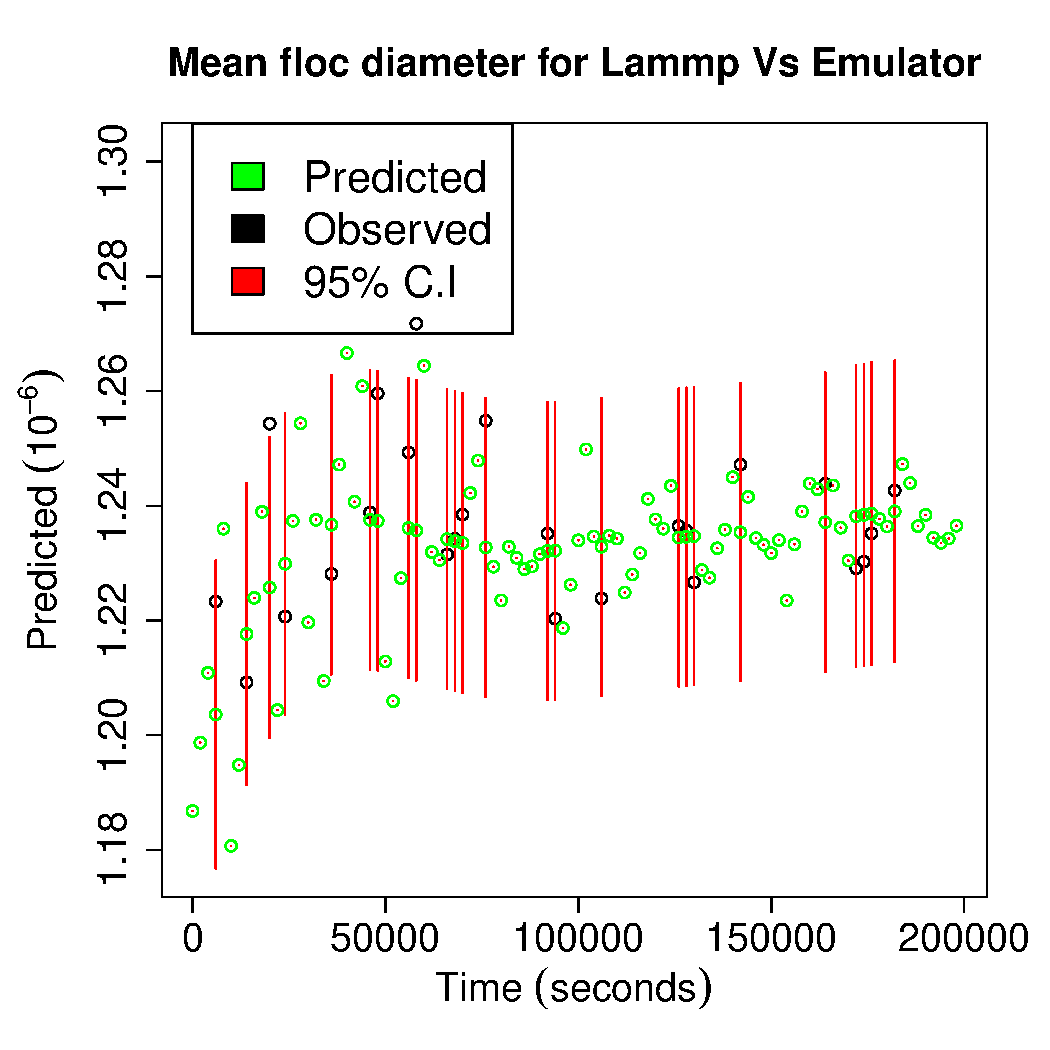
\includegraphics[height=9cm,width=1.1\textwidth]{ana/myplot5}
\caption{LAMMPS and kriging predictions at $20^{th}$ design point for all time steps. Note: The points with no C.I bands are the design points where MSE=0}
\label{myfigg9a1}
\end{subfigure}\hspace*{1em}
\begin{subfigure}[b]{.5\textwidth}
%\centering
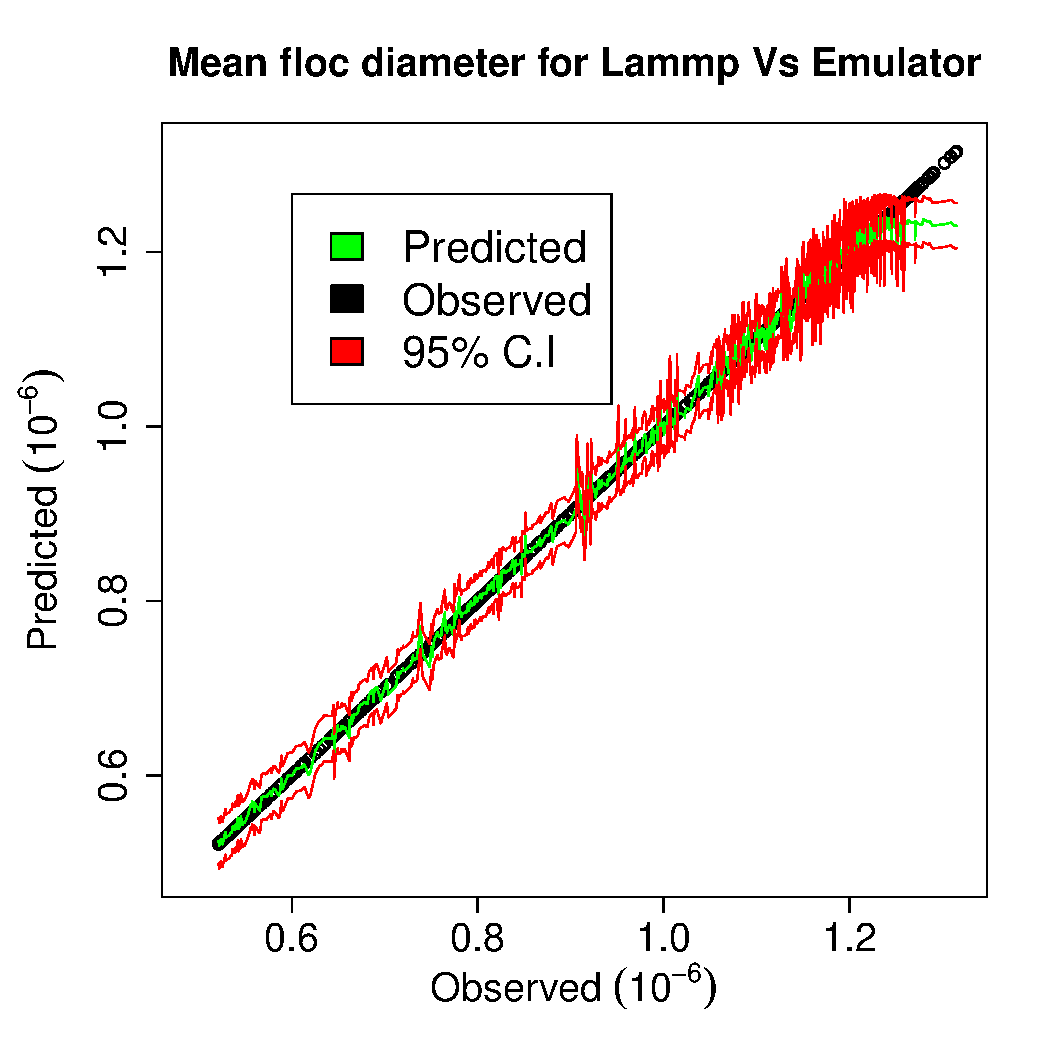
\includegraphics[height=9cm,width=1.1\textwidth]{ana/myplot3}
\caption{Pair plot for complete data set}
\label{myfigg9a2}
\end{subfigure}
\caption{Pair plot of kriging predictions (emulator) vs. LAMMPS values with their 95\% C.I for mean floc diameter (all species) using a Gaussian covariance functions}\label{myfig3}
\end{figure}

\begin{figure}[!ht] 
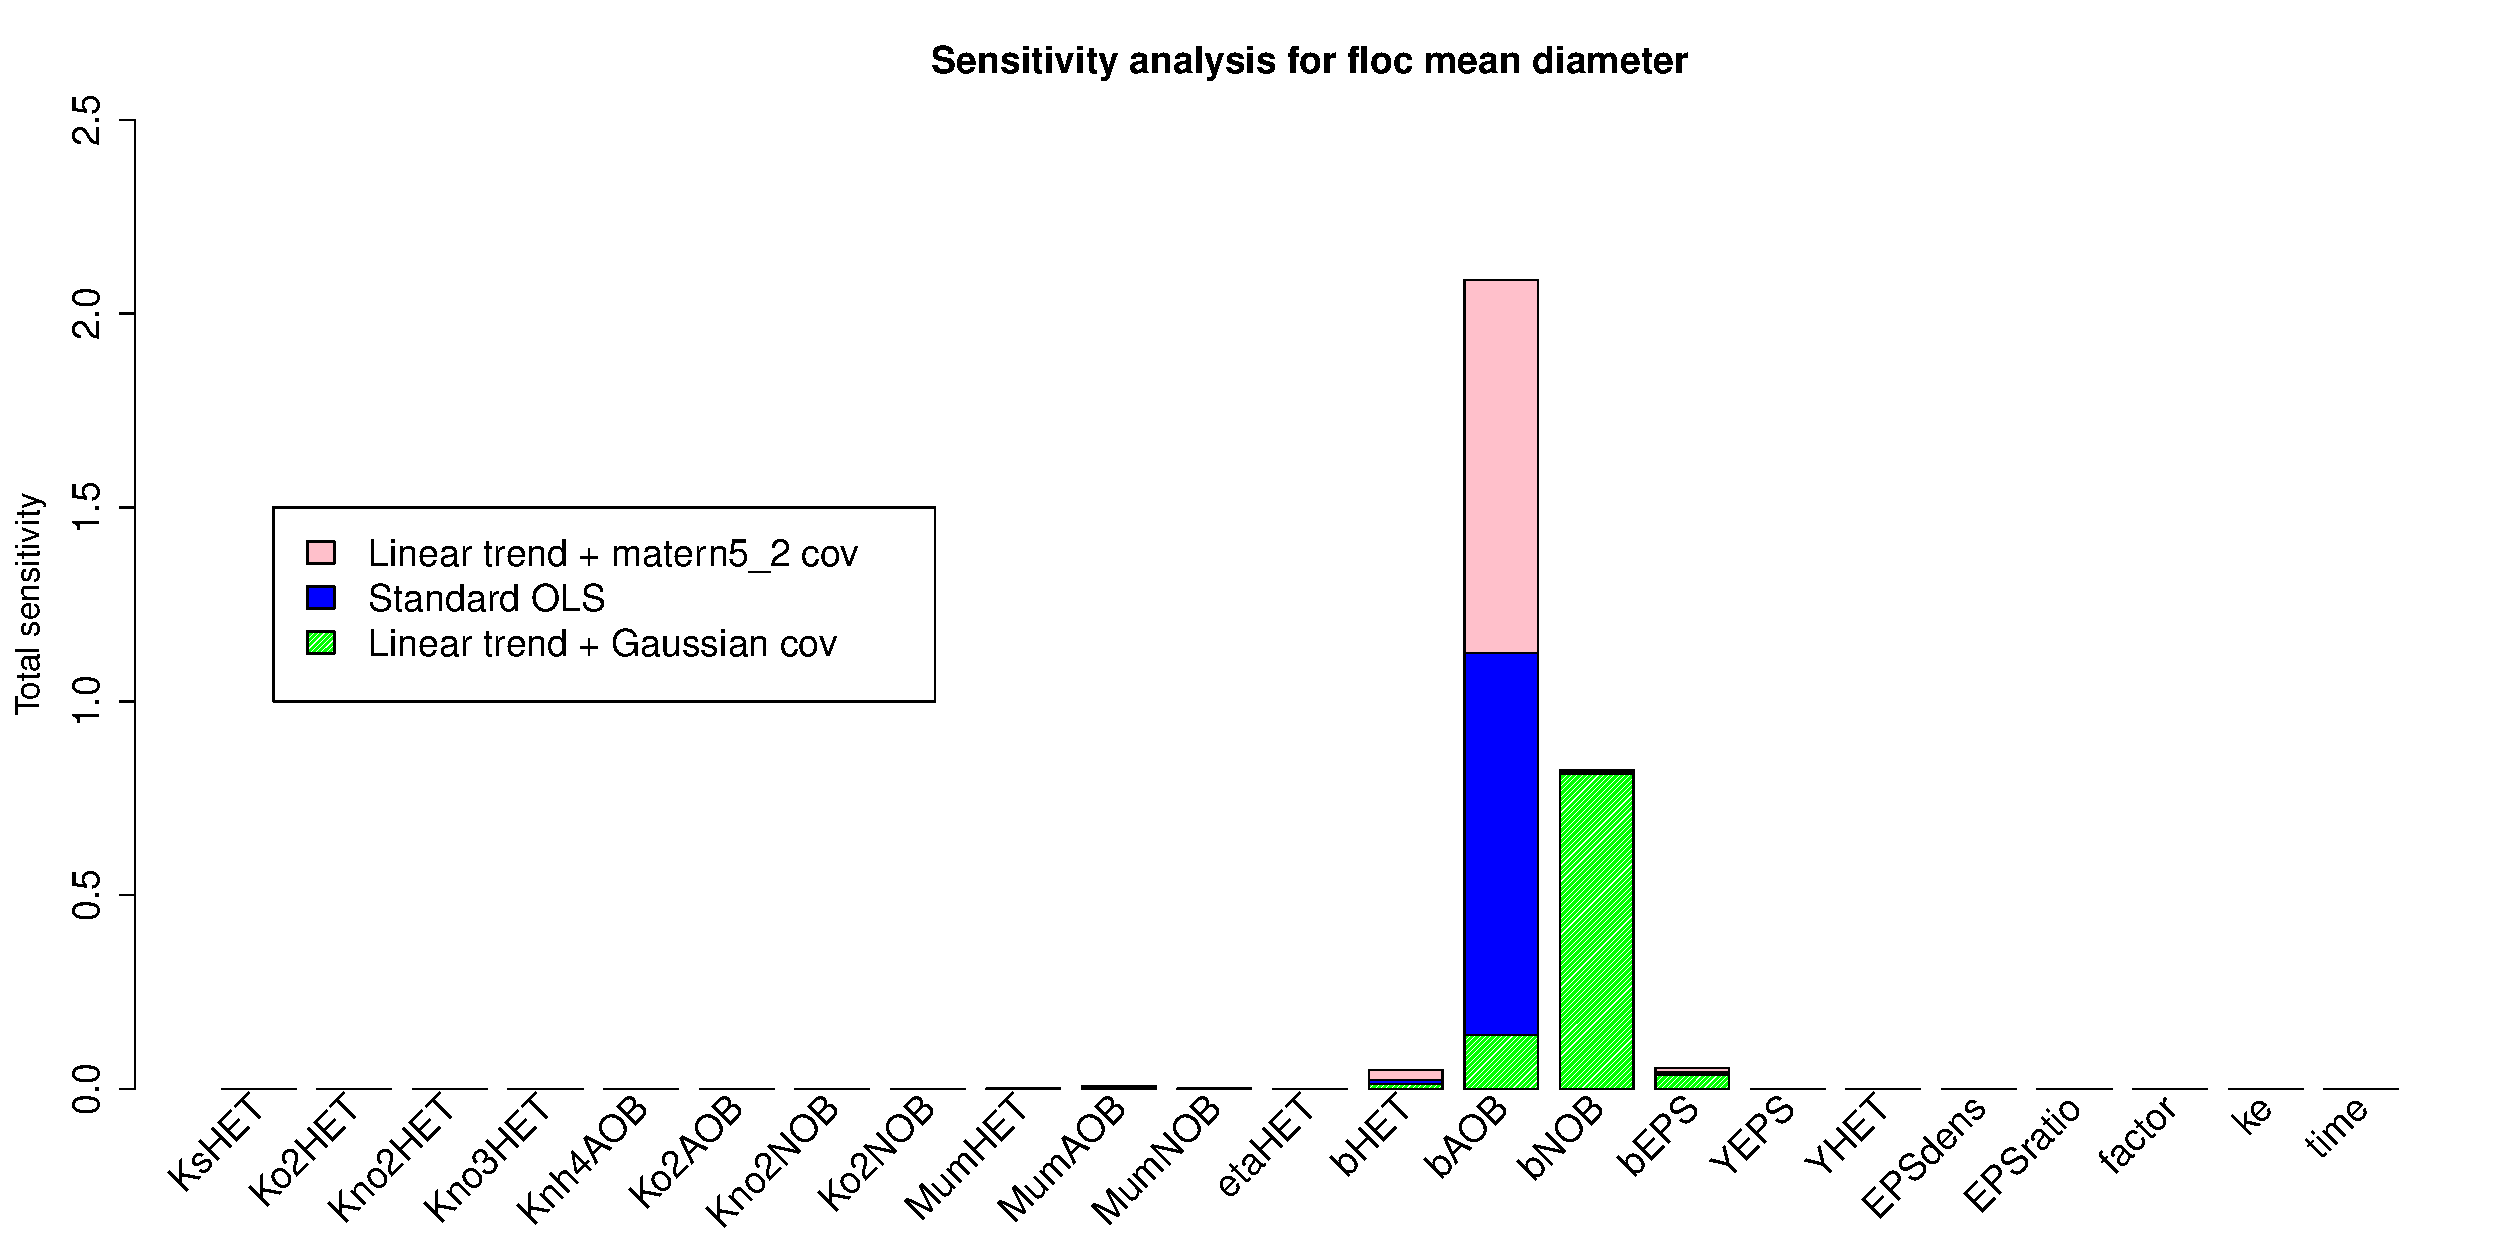
\includegraphics[width=1.1\textwidth]{ana/sensitivty_results}
\caption[]{Barplots showing total sensitivity indices for mean floc diameter using Sobol based variance decomposition technique. Comparison for three different methods.}\label{sens}
\end{figure}

%problems of optimization (cost of objective functions, numerical instabilities, multimodality and dimensionality issues)
%%%%%%
%for the fast and efficient estimation of trend and covariance parameters relying on a global optimizer with a gradient like the genoud algorithm of the package $rgenoud$
%assumed to be constructed by stepwise technique.
%Noninformative Bayesian analysis leads to kriging predictor and variance 
%appear respectively as conditional mean and variance, and the analytically tractable conditional covariance kernel enables the use of conditional simulations at any set of new design points.
%\chapter*{Appendix}

\chapter{Emulation of floc and biofilm}
The detailed procedure of emulating the floc and biofilm will be described in this section.

\begin{thebibliography}{94}
%\cleardoublepage
%\phantomsection
\bibliographystyle{plain}

\bibitem[Currin et al.(1991)]{pd1} Currin, C., Mitchell, T.J., Morris, M.D., and Ylvisaker, D. (1991). Bayesian Prediction of Deterministic Functions, With Applications to the Design and Analysis of Computer Experiments. {\it Journal of the American Statistical Association}, $86(416), 953-963$. 

\bibitem[Martin \& Simpson(2004)]{pd2} Martin, J. D., \& Simpson, T. W. (2004). On the use of kriging models to approximate deterministic computer models. {\it In ASME 2004 International Design Engineering Technical Conferences and Computers and Information in Engineering Conference}, $481-492$.

\bibitem[Osio et al.(1996)]{pd3} Osio, I.G. and Amon, C.H. (1996). An Engineering Design Methodology with Multistage Bayesian Surrogate and Optimal Sampling. {\it Research in Engineering Design}, $8(4), 189-206$.

\bibitem[Sacks et al.(1989)]{pd4} Sacks, J., Welch, W., Mitchell, T., Wynn, H. (1998). Design and analysis of computer experiments. {\it Statistical Science}, $4(4), 409-435$.

\bibitem[Santner et al.(2003)]{pd5} Santner, T., Williams, B., Notz, W. (2003). The Design and Analysis of Computer Experiments. Springer.

\bibitem[Li \& Sudjianto(2005)]{pd6} Li, R., \& Sudjianto, A. (2005). Analysis of computer experiments using penalized likelihood in gaussian kriging models. {\it Technometrics}, $47(2), 111-120$.

\bibitem[Andrianakis \& Challenor(2009)]{pd7} Andrianakis, Y., \& Challenor, P. G. (2009). Parameter estimation and prediction using Gaussian processes. {\it Technical report}, MUCM Technical Report 09/05, University of Southampton.

\bibitem[Roustant et al.(2012)]{pd8} Roustant, O., Ginsbourger, D., \& Deville, Y. (2012). DiceKriging, DiceOptim: Two R packages for the analysis of computer experiments by kriging-based metamodeling and optimization.

\bibitem[Park \& Baek(2001)]{pd9} Park J.S., \& Baek, J. (2001). Efficient Computation of Maximum Likelihood Estimators in a
Spatial Linear Model with Power Exponential Covariogram. {\it Computer Geosciences}, $27, 1-7$.

\bibitem[Hankin(2005)]{pd10} Hankin, R. K. (2005). Introducing BACCO, an R package for Bayesian analysis of computer code output. {\it Journal of Statistical Software}, $14, 16$.

\bibitem[O'Hagan(2006)]{pd11} O'Hagan, A. (2006). Bayesian Analysis of Computer Code Outputs: A Tutorial. {\it Reliability Engineering and System Safety}, $91, 1290-1300$.

\end{thebibliography}{}

\section*{Appendix 1: Estimation of prior hyperparameters}\label{hyper}
Noting that under GP regression, the prior distribution for the data is also a Gaussian distribution, the joint likelihood of the parameters is given as
\begin{equation}\tag{A.10}\label{like}
p(\boldsymbol \beta, \sigma^2, \boldsymbol{\alpha}|\by)\propto \frac{det(\bf C)^{-\frac{1}{2}}}{{(2\pi\sigma^2)}^\frac{n}{2}}\exp \Big \{\frac{(y-H\boldsymbol \beta)^T \bf C^{-1}(\by-H\boldsymbol \beta)}{2\sigma^2}\Big\}
\end{equation}
where $\boldsymbol{\alpha}=[\alpha_1, \ldots, \alpha_n]$ is a vector of correlation lengths and $det(\bf C)$ is the determinant of correlation matrix $\bf C$, integrating out $\boldsymbol \beta$ using a non-informative (uniform) prior such that $p(\boldsymbol \beta) \propto$ 1. We have a marginal likelihood
\begin{equation}\tag{A.10b}\label{like2}
p(\by|\sigma^2, \boldsymbol{\alpha})\propto \frac{\det(\bf C)^{-\frac{1}{2}}\det(H^TCH)^{-\frac{1}{2}}}{{(2\pi\sigma^2)}^\frac{n-p}{2}}\exp \Big \{\frac{(\by-\bH\hbbeta)^T \bC^{-1}(\by-\bH\hbbeta)}{2\sigma^2}\Big\}.
\end{equation}
Maximizing (\ref{like2}) with respect to $\boldsymbol \beta$ and $\sigma^2$ will give %the MLE of $\boldsymbol \beta$ 
\begin{equation}\tag{A.11}
\hbbeta=(\bH^T\bC^{-1}\bH)^{-1}\bH^T\bC^{-1}\by
%(\ref{like3})
\end{equation}

\begin{equation}\tag{A.12}
\widehat{\sigma^2}=\frac{1}{n-p}\Big[\mathbf{(y-H\hat{\boldsymbol \beta})}^T\bf C^{-1}(\bf y-H\hat{\boldsymbol \beta})\Big]
\end{equation}
Now, integrate out $\sigma^2$ such that $p(\sigma^2) \propto \frac{1}{\sigma^2}$, then we have
\begin{equation}\tag{A.10c}\label{like3}
p(\by|\boldsymbol{\alpha})\propto \det(\bC)^{-\frac{1}{2}}\det(\bH^T\bC\bH)^{-\frac{1}{2}} \Big \{(\by-\bH\hbbeta)^T \bC^{-1}(\by-\bH\hbbeta)\Big\}^{-(n-p)/2}
\end{equation}
$$=\det(\bC)^{-\frac{1}{2}}\det(\bH^T\bC\bH)^{-\frac{1}{2}} {\widehat{\sigma^2}}^{-(n-p)/2}.$$
%The smoothing parameter $\boldsymbol{\alpha}$ is estimated by maximizing the marginal likelihood (\ref{like3}) using the posterior mode%, the estimates of $\hat{\boldsymbol \beta}$ and $\widehat{\sigma^2}$ are substituted in equation (\ref{like}) and maximized over $\boldsymbol \beta$ and $\sigma^2$ to obtain


The smoothing parameter $\boldsymbol{\alpha}$ is estimated from the posterior distribution using the posterior mode by the value of $\boldsymbol{\alpha}$ for which marginal likelihood (\ref{like3}) is maximised. Here, we describe briefly the maximisation of the posterior distribution of $\boldsymbol{\alpha}$ which is reparametrized as $\btau=2log(\boldsymbol{\alpha})$ to make it unconstrained optimisation \citep{pd7, pd5}. 
Therefore, function $f(\btau)=log(p(\by|\exp(\frac{\btau}{2})))$ can be optimised using a derivative-free numerical optimisation of Nelder-Mead method which is the default in the "emulator" package that we use.
%\begin{equation}\tag{A.13}
%L(\hat{\boldsymbol \beta},\widehat{\sigma^2},\boldsymbol{\alpha})=-\frac{1}{2}\Big[n~log(\widehat{\sigma^2})(\boldsymbol{\alpha})+log(det(\bf C(\boldsymbol{\alpha})))+\textnormal n\Big],
%\end{equation}
%which is a function of $\boldsymbol{\alpha}$ that can be computed using a derivative-free numerical optimisation like Nelder-Mead method see further details in %\citep{70,q10}.
%Posterior distribution is obtained as $P(\mathbf{z}|\widehat{\boldsymbol\beta},\hat\sigma^2,\hat\alpha)\sim N[m^{\bullet}(u),\sigma^2C^{\bullet}(u,u')]$, with posterior mean and covariance functions given as equations (\ref{olu1} and \ref{olu2}) respectively.

\begin{table}
\caption{List of all the parameters}\label{mytab1}
\centering
\fbox{
\begin{tabular}{*{2}{c|c|c}}
Index&Parameters& Value\\ 
\hline
1&variable KsHET &0.01\\
2&variable Ko2HET & 0.81\\
3&variable Kno2HET & 0.0003\\
4&variable Kno3HET & 0.0003\\

5&variable Knh4AOB & 0.001\\
6&variable Ko2AOB & 0.0005\\

7&variable Kno2NOB & 0.0013\\
8&variable Ko2NOB & 0.00068\\


%#Defining maximum growth variables: list from Jaya 
9&variable MumHET & 0.00006944444\\
10&variable MumAOB & 0.00003472222\\
11&variable MumNOB & 0.00003472222\\
12&variable etaHET & 0.6\\

%#Defining decay rates variables: list from Jaya 
13&variable bHET & 0.00000462962\\
%#variable bHET & 0.00462962\\
14&variable bAOB & 0.00000127314\\
%#variable bAOB & 0.00127314\\
15&variable bNOB & 0.00000127314\\
%#variable bNOB & 0.00127314\\
16&variable bEPS & 0.00000196759\\

17&variable YEPS & 0.18\\
18&variable YHET & 0.61\\
%19&variable EPSdens & 30\\
19&variable EPSratio & 1.25\\

20&variable factor & 1.5\\
21&sub &0.08 \\
22&no2 & 0.008\\
23&no3 & 1e-05\\
24&o2 & 0.01\\
25&nh4 &0.09\\
%22&variable ke & 5e+10
\end{tabular}}
\end{table}
\end{document}
